% Informe de cierre de la fase 1 (laboratorios 1 a 3): entregable 4 de la guía 3
% Se compila con desarrollo/compilar_documentos.py (queda en laboratorios/lab03_git_y_modelo_er/)
\documentclass[a4paper,11pt]{article}
% Preámbulo común de los informes de laboratorio (II/2026). Se incluye desde desarrollo/fuentes/laboratorios/labNN_*/
%   % Preámbulo común de los informes de laboratorio (II/2026). Se incluye desde desarrollo/fuentes/laboratorios/labNN_*/
%   % Preámbulo común de los informes de laboratorio (II/2026). Se incluye desde desarrollo/fuentes/laboratorios/labNN_*/
%   \input{../informe_comun}
\input{../../gemelo-digital/manual/estilo_manual}
\input{../../gemelo-digital/manual/tecnico/macros}
% Las rutas son relativas a la carpeta de cada informe (desarrollo/fuentes/laboratorios/labNN/): las fuentes
% (estilo, imágenes del manual, figuras y levantamiento) están en desarrollo/fuentes; los entregables públicos
% (planos, base de datos) cuatro niveles más arriba, en semestres/2026_II/.
\graphicspath{{../../../../documentacion/planos_isa/pid/}{../../../../documentacion/planos_isa/electrico/}{../../../../documentacion/manuales_inversa/}
  {../../../../database/mockups/}{../../../../database/documentacion/}{../../../../database/modelo/}{../../../../database/interfaz/}
  {../../gemelo-digital/manual/img/}{../../modelo-3d/informe/figuras/}{../../modelo-3d/levantamiento/}{../../../../../../global/fotos-planta/}}
\usepackage{pdflscape}
\lstset{showstringspaces=false}
% plano A3 en una página apaisada: \plano[página]{archivo}{leyenda}
\newcommand{\plano}[3][1]{\begin{landscape}\begin{figure}[p]\centering\includegraphics[page=#1, width=\linewidth, height=0.86\textwidth, keepaspectratio]{#2}\caption{#3}\end{figure}\end{landscape}}
\setlength{\headheight}{14pt}
\newcommand{\nlab}{}
\newcommand{\tlab}{}
% tipo de documento en la portada y el encabezado (los documentos de logros los redefinen)
\newcommand{\tipodoc}{Informe del Laboratorio Integrado}
\newcommand{\tipocab}{Informe del laboratorio}
\lhead{\small Brazo XK-JS1-1 · \tipocab{} \nlab}
\rhead{\small UMSA · II/2026}

% \portada{número}{título}{inicio}{entrega}{semanas}
\newcommand{\portada}[5]{%
\renewcommand{\nlab}{#1}%
\begin{titlepage}
\centering
\vspace*{0.6cm}
{\large Universidad Mayor de San Andrés · Facultad de Ingeniería\par}
{\large Carrera de Ingeniería Electrónica\par}
\vspace{0.8cm}
{\color{naranja!80!black}\rule{\linewidth}{1.5pt}\par}
\vspace{0.3cm}
{\Large \tipodoc{} Nº #1\par}
\vspace{0.2cm}
{\huge\bfseries #2\par}
\vspace{0.3cm}
{\color{naranja!80!black}\rule{\linewidth}{1.5pt}\par}
\vspace{0.8cm}
{\large Planta: brazo robótico XK-JS1-1 de 4 grados de libertad\par}
\vspace{0.3cm}
{\large ETN-902 Sistemas de Control II · ETN-1034 Aplicación de Técnicas de Control · ETN-1000 Bases de Datos\par}
\vspace{1cm}
\begin{tabular}{rl}
\textbf{Docente:} & Ing. Jorge Antonio Nava Amador\\
\textbf{Auxiliares:} & Limber Ajnota · Fabián Plata · Franz Choque\\
\textbf{Inicio de trabajo:} & #3\\
\textbf{Entrega:} & #4 (#5)\\
\end{tabular}
\vspace{1cm}

\begin{tabular}{ll}
\multicolumn{2}{l}{\textbf{Escuadra del brazo de 4 GDL}}\\[2pt]
Control (ETN-902 / ETN-1034): & Gabriel Andres Gomez Calla\\
 & Jose Lenin Mamani Choque\\
 & Miguel Alejandro Lima Huarachi\\
 & Román Abner Machicado Arequipa\\[2pt]
Cómputo (ETN-1000): & Miguel Alejandro Lima Huarachi\\
 & Marco Eduardo Chura Rondo\\
\end{tabular}
\vfill
{\small Repositorio: \url{https://github.com/GabAndGom/Brazo-de-4-grados-de-libertad}\par}
{\small La Paz, Bolivia · gestión II/2026\par}
\end{titlepage}
}

% Tabla de entregables (Definition of Done): \begin{dod} ... \end{dod}, filas: entregable & estado & evidencia\\
\newenvironment{dod}{\begin{center}\small\begin{longtable}{>{\raggedright}p{5.2cm} >{\raggedright}p{1.8cm} >{\raggedright\arraybackslash}p{7.6cm}}
\toprule \textbf{Entregable} & \textbf{Estado} & \textbf{Evidencia / observación}\\ \midrule \endhead}
{\bottomrule\end{longtable}\end{center}}

% Estilo común de los manuales del gemelo digital (se incluye con \input)
\usepackage{geometry}
\geometry{letterpaper, margin=2.2cm}
\usepackage[spanish, es-nodecimaldot, mexico]{babel}
\usepackage[utf8]{inputenc}
\usepackage[T1]{fontenc}
\usepackage{lmodern}
\usepackage{amsmath,amssymb}
\usepackage[table]{xcolor}
\definecolor{naranja}{RGB}{194,98,12}
\definecolor{rojo}{RGB}{192,57,43}
\definecolor{verde}{RGB}{30,120,70}
\definecolor{azulw}{RGB}{0,103,184}
\definecolor{azulg}{RGB}{70,90,120}
\definecolor{gris}{RGB}{242,242,242}
\definecolor{grisos}{RGB}{90,90,90}
\usepackage{booktabs,longtable,array,tabularx}
\usepackage{graphicx}
\usepackage{float}
\usepackage{caption}
\captionsetup{font=small, labelfont=bf}
\usepackage{tikz}
\usetikzlibrary{positioning,arrows.meta,fit,calc,shapes.geometric,decorations.pathreplacing,backgrounds}
\usepackage{enumitem}
\setlist{itemsep=2pt}
\usepackage{listings}
\lstset{basicstyle=\ttfamily\small, frame=single, backgroundcolor=\color{gris}, breaklines=true,
  columns=fullflexible, keepspaces=true, extendedchars=true, upquote=true,
  literate={á}{{\'a}}1 {é}{{\'e}}1 {í}{{\'i}}1 {ó}{{\'o}}1 {ú}{{\'u}}1 {ñ}{{\~n}}1 {Á}{{\'A}}1 {É}{{\'E}}1
           {Í}{{\'I}}1 {Ó}{{\'O}}1 {Ú}{{\'U}}1 {Ñ}{{\~N}}1 {ü}{{\"u}}1 {¿}{{?`}}1 {¡}{{!`}}1 {…}{{...}}3
           {θ}{{$\theta$}}1 {·}{{$\cdot$}}1 {«}{{\guillemotleft}}1 {»}{{\guillemotright}}1 {°}{{$^\circ$}}1}
\usepackage{hyperref}
\hypersetup{colorlinks=true, linkcolor=naranja, urlcolor=naranja}
\usepackage{fancyhdr}
\pagestyle{fancy}
\fancyhf{}
\cfoot{\small \thepage}
\newcommand{\codigo}[1]{\texttt{#1}}
\newcommand{\archivo}[1]{\textbf{\texttt{#1}}}
\newcommand{\aviso}[1]{\par\smallskip\noindent\colorbox{rojo!10}{\parbox{\dimexpr\linewidth-2\fboxsep}{\textbf{\color{rojo}Atención.} #1}}\par\smallskip}
\newcommand{\nota}[1]{\par\smallskip\noindent\colorbox{gris}{\parbox{\dimexpr\linewidth-2\fboxsep}{#1}}\par\smallskip}
\tikzset{
  marca/.style={circle, fill=naranja, text=white, font=\bfseries\footnotesize, inner sep=1.4pt, minimum size=4.6mm, draw=white, line width=0.8pt},
  caja/.style={draw, rounded corners=2pt, fill=gris, align=center, font=\small, minimum height=10mm, inner sep=4pt},
  cajab/.style={caja, fill=white},
  cajan/.style={caja, fill=naranja!14, draw=naranja!70!black},
  paso/.style={draw, rounded corners=2pt, fill=white, align=left, font=\small, text width=3.4cm, minimum height=15mm, inner sep=5pt},
  num/.style={circle, fill=naranja, text=white, font=\bfseries\small, inner sep=1.5pt, minimum size=6mm},
  flecha/.style={-{Stealth[length=2.2mm]}, thick},
  dflecha/.style={{Stealth[length=2.2mm]}-{Stealth[length=2.2mm]}, thick},
  etiq/.style={font=\scriptsize, align=center},
}
\DeclareRobustCommand{\num}[1]{\tikz[baseline=-0.7ex]\node[marca]{#1};}
% \captura{ancho}{archivo}{marcas en coordenadas 0-1 desde la esquina inferior izquierda}
\newcommand{\captura}[3]{%
  \begin{tikzpicture}
  \node[anchor=south west, inner sep=0, draw=black!25] (img) {\includegraphics[width=#1]{#2}};
  \begin{scope}[x={(img.south east)}, y={(img.north west)}]
  #3
  \end{scope}
  \end{tikzpicture}}
% ventana dibujada (consolas y diálogos): \ventana{ancho}{alto}{título}{contenido}
\newcommand{\ventana}[4]{%
\begin{tikzpicture}
\node[draw=black!50, fill=white, minimum width=#1, minimum height=#2, anchor=north west, inner sep=0] (v) at (0,0) {};
\fill[black!8] (v.north west) rectangle ($(v.north east)+(0,-6mm)$);
\node[anchor=west, font=\scriptsize] at ($(v.north west)+(2mm,-3mm)$) {#3};
\node[anchor=east, font=\scriptsize] at ($(v.north east)+(-2mm,-3mm)$) {--\quad$\square$\quad$\times$};
\node[anchor=north west, inner sep=3mm, text width=#1-6mm, font=\scriptsize\ttfamily, align=left] at ($(v.north west)+(0,-6mm)$) {#4};
\end{tikzpicture}}

% Macros del manual técnico: ladder, estados, código y rutas de imágenes
\usetikzlibrary{shapes.multipart}
\graphicspath{{../img/}{../../../../../../../global/fotos-planta/}{../../../modelo-3d/informe/figuras/}{../../../modelo-3d/levantamiento/}{../../../../../database/modelo/}{../../../../../documentacion/manuales_inversa/}{../../../../../documentacion/planos_isa/electrico/}{../../../../../database/interfaz/}}

\lstdefinestyle{py}{language=Python, keywordstyle=\color{azulg}\bfseries, commentstyle=\color{grisos}\itshape,
  stringstyle=\color{verde}, basicstyle=\ttfamily\scriptsize, numbers=left, numberstyle=\tiny\color{grisos}}
\lstdefinestyle{js}{language=Java, morekeywords={const,let,function,async,await,return,for,of,if,else}, keywordstyle=\color{azulg}\bfseries,
  commentstyle=\color{grisos}\itshape, stringstyle=\color{verde}, basicstyle=\ttfamily\scriptsize, numbers=left, numberstyle=\tiny\color{grisos}}
\lstdefinestyle{awl}{basicstyle=\ttfamily\tiny, commentstyle=\color{grisos}\itshape, morecomment=[l]{//},
  keywordstyle=\color{azulg}\bfseries, morekeywords={LD,LDN,A,AN,O,ON,EU,ED,S,R,MOVB,MOVW,MOVD,PLS,TON,CALL,CRET,LPS,LRD,LPP,ALD,OLD,FILL,LDW,LDB,LDD,AW,AD,AB,OW,OD},
  numbers=left, numberstyle=\tiny\color{grisos}, frame=single, backgroundcolor=\color{gris}}
\lstdefinestyle{sql}{language=SQL, keywordstyle=\color{azulg}\bfseries, commentstyle=\color{grisos}\itshape,
  stringstyle=\color{verde}, basicstyle=\ttfamily\tiny, numbers=left, numberstyle=\tiny\color{grisos},
  morekeywords={REFERENCES,SERIAL,SMALLSERIAL,BIGSERIAL,TIMESTAMPTZ,BOOLEAN,INET,RETURNS,TRIGGER,LANGUAGE,DECLARE,RAISE,EXCEPTION,VIEW,INDEX}}

\tikzset{
  ld/.style={line width=0.7pt},
  pics/na/.style={code={\fill[white](-0.12,-0.26) rectangle (0.12,0.26);
     \draw[thick](-0.1,-0.24)--(-0.1,0.24)(0.1,-0.24)--(0.1,0.24);
     \node[font=\scriptsize\ttfamily, above] at (0,0.22){#1};}},
  pics/nc/.style={code={\fill[white](-0.12,-0.26) rectangle (0.12,0.26);
     \draw[thick](-0.1,-0.24)--(-0.1,0.24)(0.1,-0.24)--(0.1,0.24);\draw(-0.17,-0.24)--(0.17,0.24);
     \node[font=\scriptsize\ttfamily, above] at (0,0.22){#1};}},
  pics/pf/.style={code={\fill[white](-0.12,-0.26) rectangle (0.12,0.26);
     \draw[thick](-0.1,-0.24)--(-0.1,0.24)(0.1,-0.24)--(0.1,0.24);
     \node[font=\tiny\bfseries] at (0,0){P};}},
  pics/cmp/.style n args={3}{code={\fill[white](-0.12,-0.26) rectangle (0.12,0.26);
     \draw[thick](-0.1,-0.24)--(-0.1,0.24)(0.1,-0.24)--(0.1,0.24);
     \node[font=\tiny\ttfamily] at (0,0){#2};
     \node[font=\scriptsize\ttfamily, above] at (0,0.22){#1};
     \node[font=\scriptsize\ttfamily, below] at (0,-0.22){#3};}},
  pics/bob/.style n args={3}{code={\fill[white](-0.2,-0.26) rectangle (0.2,0.26);
     \draw[thick](-0.05,0.24) arc (110:250:0.255);\draw[thick](0.05,0.24) arc (70:-70:0.255);
     \node[font=\tiny\bfseries] at (0,0){#2};
     \node[font=\scriptsize\ttfamily, above] at (0,0.22){#1};
     \node[font=\scriptsize\ttfamily, below] at (0,-0.22){#3};}},
  fb/.style={draw, fill=white, font=\scriptsize\ttfamily, align=left, inner sep=3pt, anchor=west},
  barra/.style={line width=2pt},
  estado/.style={draw, rounded corners=3pt, fill=white, align=center, font=\scriptsize, minimum width=22mm, minimum height=10mm, inner sep=3pt},
  estadon/.style={estado, fill=naranja!14, draw=naranja!70!black},
  trans/.style={font=\scriptsize, align=center, fill=white, inner sep=1pt},
  lugar/.style={circle, draw, thick, minimum size=7mm, fill=white},
  transicion/.style={rectangle, fill=black, minimum width=1.6mm, minimum height=7mm, inner sep=0},
  tabla/.style={rectangle split, rectangle split parts=2, draw, fill=white, font=\tiny\ttfamily, align=left, inner sep=2pt, rounded corners=1pt, text width=33mm},
}
\newcommand{\pendiente}[1]{\par\smallskip\noindent\colorbox{naranja!12}{\parbox{\dimexpr\linewidth-2\fboxsep}{\textbf{\color{naranja!80!black}Pendiente.} #1}}\par\smallskip}
\newcommand{\cumple}{\textcolor{verde}{\textbf{cumplido}}}
\newcommand{\parcial}{\textcolor{naranja}{\textbf{parcial}}}
\newcommand{\falta}{\textcolor{rojo}{\textbf{pendiente}}}

% Las rutas son relativas a la carpeta de cada informe (desarrollo/fuentes/laboratorios/labNN/): las fuentes
% (estilo, imágenes del manual, figuras y levantamiento) están en desarrollo/fuentes; los entregables públicos
% (planos, base de datos) cuatro niveles más arriba, en semestres/2026_II/.
\graphicspath{{../../../../documentacion/planos_isa/pid/}{../../../../documentacion/planos_isa/electrico/}{../../../../documentacion/manuales_inversa/}
  {../../../../database/mockups/}{../../../../database/documentacion/}{../../../../database/modelo/}{../../../../database/interfaz/}
  {../../gemelo-digital/manual/img/}{../../modelo-3d/informe/figuras/}{../../modelo-3d/levantamiento/}{../../../../../../global/fotos-planta/}}
\usepackage{pdflscape}
\lstset{showstringspaces=false}
% plano A3 en una página apaisada: \plano[página]{archivo}{leyenda}
\newcommand{\plano}[3][1]{\begin{landscape}\begin{figure}[p]\centering\includegraphics[page=#1, width=\linewidth, height=0.86\textwidth, keepaspectratio]{#2}\caption{#3}\end{figure}\end{landscape}}
\setlength{\headheight}{14pt}
\newcommand{\nlab}{}
\newcommand{\tlab}{}
% tipo de documento en la portada y el encabezado (los documentos de logros los redefinen)
\newcommand{\tipodoc}{Informe del Laboratorio Integrado}
\newcommand{\tipocab}{Informe del laboratorio}
\lhead{\small Brazo XK-JS1-1 · \tipocab{} \nlab}
\rhead{\small UMSA · II/2026}

% \portada{número}{título}{inicio}{entrega}{semanas}
\newcommand{\portada}[5]{%
\renewcommand{\nlab}{#1}%
\begin{titlepage}
\centering
\vspace*{0.6cm}
{\large Universidad Mayor de San Andrés · Facultad de Ingeniería\par}
{\large Carrera de Ingeniería Electrónica\par}
\vspace{0.8cm}
{\color{naranja!80!black}\rule{\linewidth}{1.5pt}\par}
\vspace{0.3cm}
{\Large \tipodoc{} Nº #1\par}
\vspace{0.2cm}
{\huge\bfseries #2\par}
\vspace{0.3cm}
{\color{naranja!80!black}\rule{\linewidth}{1.5pt}\par}
\vspace{0.8cm}
{\large Planta: brazo robótico XK-JS1-1 de 4 grados de libertad\par}
\vspace{0.3cm}
{\large ETN-902 Sistemas de Control II · ETN-1034 Aplicación de Técnicas de Control · ETN-1000 Bases de Datos\par}
\vspace{1cm}
\begin{tabular}{rl}
\textbf{Docente:} & Ing. Jorge Antonio Nava Amador\\
\textbf{Auxiliares:} & Limber Ajnota · Fabián Plata · Franz Choque\\
\textbf{Inicio de trabajo:} & #3\\
\textbf{Entrega:} & #4 (#5)\\
\end{tabular}
\vspace{1cm}

\begin{tabular}{ll}
\multicolumn{2}{l}{\textbf{Escuadra del brazo de 4 GDL}}\\[2pt]
Control (ETN-902 / ETN-1034): & Gabriel Andres Gomez Calla\\
 & Jose Lenin Mamani Choque\\
 & Miguel Alejandro Lima Huarachi\\
 & Román Abner Machicado Arequipa\\[2pt]
Cómputo (ETN-1000): & Miguel Alejandro Lima Huarachi\\
 & Marco Eduardo Chura Rondo\\
\end{tabular}
\vfill
{\small Repositorio: \url{https://github.com/GabAndGom/Brazo-de-4-grados-de-libertad}\par}
{\small La Paz, Bolivia · gestión II/2026\par}
\end{titlepage}
}

% Tabla de entregables (Definition of Done): \begin{dod} ... \end{dod}, filas: entregable & estado & evidencia\\
\newenvironment{dod}{\begin{center}\small\begin{longtable}{>{\raggedright}p{5.2cm} >{\raggedright}p{1.8cm} >{\raggedright\arraybackslash}p{7.6cm}}
\toprule \textbf{Entregable} & \textbf{Estado} & \textbf{Evidencia / observación}\\ \midrule \endhead}
{\bottomrule\end{longtable}\end{center}}

% Estilo común de los manuales del gemelo digital (se incluye con \input)
\usepackage{geometry}
\geometry{letterpaper, margin=2.2cm}
\usepackage[spanish, es-nodecimaldot, mexico]{babel}
\usepackage[utf8]{inputenc}
\usepackage[T1]{fontenc}
\usepackage{lmodern}
\usepackage{amsmath,amssymb}
\usepackage[table]{xcolor}
\definecolor{naranja}{RGB}{194,98,12}
\definecolor{rojo}{RGB}{192,57,43}
\definecolor{verde}{RGB}{30,120,70}
\definecolor{azulw}{RGB}{0,103,184}
\definecolor{azulg}{RGB}{70,90,120}
\definecolor{gris}{RGB}{242,242,242}
\definecolor{grisos}{RGB}{90,90,90}
\usepackage{booktabs,longtable,array,tabularx}
\usepackage{graphicx}
\usepackage{float}
\usepackage{caption}
\captionsetup{font=small, labelfont=bf}
\usepackage{tikz}
\usetikzlibrary{positioning,arrows.meta,fit,calc,shapes.geometric,decorations.pathreplacing,backgrounds}
\usepackage{enumitem}
\setlist{itemsep=2pt}
\usepackage{listings}
\lstset{basicstyle=\ttfamily\small, frame=single, backgroundcolor=\color{gris}, breaklines=true,
  columns=fullflexible, keepspaces=true, extendedchars=true, upquote=true,
  literate={á}{{\'a}}1 {é}{{\'e}}1 {í}{{\'i}}1 {ó}{{\'o}}1 {ú}{{\'u}}1 {ñ}{{\~n}}1 {Á}{{\'A}}1 {É}{{\'E}}1
           {Í}{{\'I}}1 {Ó}{{\'O}}1 {Ú}{{\'U}}1 {Ñ}{{\~N}}1 {ü}{{\"u}}1 {¿}{{?`}}1 {¡}{{!`}}1 {…}{{...}}3
           {θ}{{$\theta$}}1 {·}{{$\cdot$}}1 {«}{{\guillemotleft}}1 {»}{{\guillemotright}}1 {°}{{$^\circ$}}1}
\usepackage{hyperref}
\hypersetup{colorlinks=true, linkcolor=naranja, urlcolor=naranja}
\usepackage{fancyhdr}
\pagestyle{fancy}
\fancyhf{}
\cfoot{\small \thepage}
\newcommand{\codigo}[1]{\texttt{#1}}
\newcommand{\archivo}[1]{\textbf{\texttt{#1}}}
\newcommand{\aviso}[1]{\par\smallskip\noindent\colorbox{rojo!10}{\parbox{\dimexpr\linewidth-2\fboxsep}{\textbf{\color{rojo}Atención.} #1}}\par\smallskip}
\newcommand{\nota}[1]{\par\smallskip\noindent\colorbox{gris}{\parbox{\dimexpr\linewidth-2\fboxsep}{#1}}\par\smallskip}
\tikzset{
  marca/.style={circle, fill=naranja, text=white, font=\bfseries\footnotesize, inner sep=1.4pt, minimum size=4.6mm, draw=white, line width=0.8pt},
  caja/.style={draw, rounded corners=2pt, fill=gris, align=center, font=\small, minimum height=10mm, inner sep=4pt},
  cajab/.style={caja, fill=white},
  cajan/.style={caja, fill=naranja!14, draw=naranja!70!black},
  paso/.style={draw, rounded corners=2pt, fill=white, align=left, font=\small, text width=3.4cm, minimum height=15mm, inner sep=5pt},
  num/.style={circle, fill=naranja, text=white, font=\bfseries\small, inner sep=1.5pt, minimum size=6mm},
  flecha/.style={-{Stealth[length=2.2mm]}, thick},
  dflecha/.style={{Stealth[length=2.2mm]}-{Stealth[length=2.2mm]}, thick},
  etiq/.style={font=\scriptsize, align=center},
}
\DeclareRobustCommand{\num}[1]{\tikz[baseline=-0.7ex]\node[marca]{#1};}
% \captura{ancho}{archivo}{marcas en coordenadas 0-1 desde la esquina inferior izquierda}
\newcommand{\captura}[3]{%
  \begin{tikzpicture}
  \node[anchor=south west, inner sep=0, draw=black!25] (img) {\includegraphics[width=#1]{#2}};
  \begin{scope}[x={(img.south east)}, y={(img.north west)}]
  #3
  \end{scope}
  \end{tikzpicture}}
% ventana dibujada (consolas y diálogos): \ventana{ancho}{alto}{título}{contenido}
\newcommand{\ventana}[4]{%
\begin{tikzpicture}
\node[draw=black!50, fill=white, minimum width=#1, minimum height=#2, anchor=north west, inner sep=0] (v) at (0,0) {};
\fill[black!8] (v.north west) rectangle ($(v.north east)+(0,-6mm)$);
\node[anchor=west, font=\scriptsize] at ($(v.north west)+(2mm,-3mm)$) {#3};
\node[anchor=east, font=\scriptsize] at ($(v.north east)+(-2mm,-3mm)$) {--\quad$\square$\quad$\times$};
\node[anchor=north west, inner sep=3mm, text width=#1-6mm, font=\scriptsize\ttfamily, align=left] at ($(v.north west)+(0,-6mm)$) {#4};
\end{tikzpicture}}

% Macros del manual técnico: ladder, estados, código y rutas de imágenes
\usetikzlibrary{shapes.multipart}
\graphicspath{{../img/}{../../../../../../../global/fotos-planta/}{../../../modelo-3d/informe/figuras/}{../../../modelo-3d/levantamiento/}{../../../../../database/modelo/}{../../../../../documentacion/manuales_inversa/}{../../../../../documentacion/planos_isa/electrico/}{../../../../../database/interfaz/}}

\lstdefinestyle{py}{language=Python, keywordstyle=\color{azulg}\bfseries, commentstyle=\color{grisos}\itshape,
  stringstyle=\color{verde}, basicstyle=\ttfamily\scriptsize, numbers=left, numberstyle=\tiny\color{grisos}}
\lstdefinestyle{js}{language=Java, morekeywords={const,let,function,async,await,return,for,of,if,else}, keywordstyle=\color{azulg}\bfseries,
  commentstyle=\color{grisos}\itshape, stringstyle=\color{verde}, basicstyle=\ttfamily\scriptsize, numbers=left, numberstyle=\tiny\color{grisos}}
\lstdefinestyle{awl}{basicstyle=\ttfamily\tiny, commentstyle=\color{grisos}\itshape, morecomment=[l]{//},
  keywordstyle=\color{azulg}\bfseries, morekeywords={LD,LDN,A,AN,O,ON,EU,ED,S,R,MOVB,MOVW,MOVD,PLS,TON,CALL,CRET,LPS,LRD,LPP,ALD,OLD,FILL,LDW,LDB,LDD,AW,AD,AB,OW,OD},
  numbers=left, numberstyle=\tiny\color{grisos}, frame=single, backgroundcolor=\color{gris}}
\lstdefinestyle{sql}{language=SQL, keywordstyle=\color{azulg}\bfseries, commentstyle=\color{grisos}\itshape,
  stringstyle=\color{verde}, basicstyle=\ttfamily\tiny, numbers=left, numberstyle=\tiny\color{grisos},
  morekeywords={REFERENCES,SERIAL,SMALLSERIAL,BIGSERIAL,TIMESTAMPTZ,BOOLEAN,INET,RETURNS,TRIGGER,LANGUAGE,DECLARE,RAISE,EXCEPTION,VIEW,INDEX}}

\tikzset{
  ld/.style={line width=0.7pt},
  pics/na/.style={code={\fill[white](-0.12,-0.26) rectangle (0.12,0.26);
     \draw[thick](-0.1,-0.24)--(-0.1,0.24)(0.1,-0.24)--(0.1,0.24);
     \node[font=\scriptsize\ttfamily, above] at (0,0.22){#1};}},
  pics/nc/.style={code={\fill[white](-0.12,-0.26) rectangle (0.12,0.26);
     \draw[thick](-0.1,-0.24)--(-0.1,0.24)(0.1,-0.24)--(0.1,0.24);\draw(-0.17,-0.24)--(0.17,0.24);
     \node[font=\scriptsize\ttfamily, above] at (0,0.22){#1};}},
  pics/pf/.style={code={\fill[white](-0.12,-0.26) rectangle (0.12,0.26);
     \draw[thick](-0.1,-0.24)--(-0.1,0.24)(0.1,-0.24)--(0.1,0.24);
     \node[font=\tiny\bfseries] at (0,0){P};}},
  pics/cmp/.style n args={3}{code={\fill[white](-0.12,-0.26) rectangle (0.12,0.26);
     \draw[thick](-0.1,-0.24)--(-0.1,0.24)(0.1,-0.24)--(0.1,0.24);
     \node[font=\tiny\ttfamily] at (0,0){#2};
     \node[font=\scriptsize\ttfamily, above] at (0,0.22){#1};
     \node[font=\scriptsize\ttfamily, below] at (0,-0.22){#3};}},
  pics/bob/.style n args={3}{code={\fill[white](-0.2,-0.26) rectangle (0.2,0.26);
     \draw[thick](-0.05,0.24) arc (110:250:0.255);\draw[thick](0.05,0.24) arc (70:-70:0.255);
     \node[font=\tiny\bfseries] at (0,0){#2};
     \node[font=\scriptsize\ttfamily, above] at (0,0.22){#1};
     \node[font=\scriptsize\ttfamily, below] at (0,-0.22){#3};}},
  fb/.style={draw, fill=white, font=\scriptsize\ttfamily, align=left, inner sep=3pt, anchor=west},
  barra/.style={line width=2pt},
  estado/.style={draw, rounded corners=3pt, fill=white, align=center, font=\scriptsize, minimum width=22mm, minimum height=10mm, inner sep=3pt},
  estadon/.style={estado, fill=naranja!14, draw=naranja!70!black},
  trans/.style={font=\scriptsize, align=center, fill=white, inner sep=1pt},
  lugar/.style={circle, draw, thick, minimum size=7mm, fill=white},
  transicion/.style={rectangle, fill=black, minimum width=1.6mm, minimum height=7mm, inner sep=0},
  tabla/.style={rectangle split, rectangle split parts=2, draw, fill=white, font=\tiny\ttfamily, align=left, inner sep=2pt, rounded corners=1pt, text width=33mm},
}
\newcommand{\pendiente}[1]{\par\smallskip\noindent\colorbox{naranja!12}{\parbox{\dimexpr\linewidth-2\fboxsep}{\textbf{\color{naranja!80!black}Pendiente.} #1}}\par\smallskip}
\newcommand{\cumple}{\textcolor{verde}{\textbf{cumplido}}}
\newcommand{\parcial}{\textcolor{naranja}{\textbf{parcial}}}
\newcommand{\falta}{\textcolor{rojo}{\textbf{pendiente}}}

% Las rutas son relativas a la carpeta de cada informe (desarrollo/fuentes/laboratorios/labNN/): las fuentes
% (estilo, imágenes del manual, figuras y levantamiento) están en desarrollo/fuentes; los entregables públicos
% (planos, base de datos) cuatro niveles más arriba, en semestres/2026_II/.
\graphicspath{{../../../../documentacion/planos_isa/pid/}{../../../../documentacion/planos_isa/electrico/}{../../../../documentacion/manuales_inversa/}
  {../../../../database/mockups/}{../../../../database/documentacion/}{../../../../database/modelo/}{../../../../database/interfaz/}
  {../../gemelo-digital/manual/img/}{../../modelo-3d/informe/figuras/}{../../modelo-3d/levantamiento/}{../../../../../../global/fotos-planta/}}
\usepackage{pdflscape}
\lstset{showstringspaces=false}
% plano A3 en una página apaisada: \plano[página]{archivo}{leyenda}
\newcommand{\plano}[3][1]{\begin{landscape}\begin{figure}[p]\centering\includegraphics[page=#1, width=\linewidth, height=0.86\textwidth, keepaspectratio]{#2}\caption{#3}\end{figure}\end{landscape}}
\setlength{\headheight}{14pt}
\newcommand{\nlab}{}
\newcommand{\tlab}{}
% tipo de documento en la portada y el encabezado (los documentos de logros los redefinen)
\newcommand{\tipodoc}{Informe del Laboratorio Integrado}
\newcommand{\tipocab}{Informe del laboratorio}
\lhead{\small Brazo XK-JS1-1 · \tipocab{} \nlab}
\rhead{\small UMSA · II/2026}

% \portada{número}{título}{inicio}{entrega}{semanas}
\newcommand{\portada}[5]{%
\renewcommand{\nlab}{#1}%
\begin{titlepage}
\centering
\vspace*{0.6cm}
{\large Universidad Mayor de San Andrés · Facultad de Ingeniería\par}
{\large Carrera de Ingeniería Electrónica\par}
\vspace{0.8cm}
{\color{naranja!80!black}\rule{\linewidth}{1.5pt}\par}
\vspace{0.3cm}
{\Large \tipodoc{} Nº #1\par}
\vspace{0.2cm}
{\huge\bfseries #2\par}
\vspace{0.3cm}
{\color{naranja!80!black}\rule{\linewidth}{1.5pt}\par}
\vspace{0.8cm}
{\large Planta: brazo robótico XK-JS1-1 de 4 grados de libertad\par}
\vspace{0.3cm}
{\large ETN-902 Sistemas de Control II · ETN-1034 Aplicación de Técnicas de Control · ETN-1000 Bases de Datos\par}
\vspace{1cm}
\begin{tabular}{rl}
\textbf{Docente:} & Ing. Jorge Antonio Nava Amador\\
\textbf{Auxiliares:} & Limber Ajnota · Fabián Plata · Franz Choque\\
\textbf{Inicio de trabajo:} & #3\\
\textbf{Entrega:} & #4 (#5)\\
\end{tabular}
\vspace{1cm}

\begin{tabular}{ll}
\multicolumn{2}{l}{\textbf{Escuadra del brazo de 4 GDL}}\\[2pt]
Control (ETN-902 / ETN-1034): & Gabriel Andres Gomez Calla\\
 & Jose Lenin Mamani Choque\\
 & Miguel Alejandro Lima Huarachi\\
 & Román Abner Machicado Arequipa\\[2pt]
Cómputo (ETN-1000): & Miguel Alejandro Lima Huarachi\\
 & Marco Eduardo Chura Rondo\\
\end{tabular}
\vfill
{\small Repositorio: \url{https://github.com/GabAndGom/Brazo-de-4-grados-de-libertad}\par}
{\small La Paz, Bolivia · gestión II/2026\par}
\end{titlepage}
}

% Tabla de entregables (Definition of Done): \begin{dod} ... \end{dod}, filas: entregable & estado & evidencia\\
\newenvironment{dod}{\begin{center}\small\begin{longtable}{>{\raggedright}p{5.2cm} >{\raggedright}p{1.8cm} >{\raggedright\arraybackslash}p{7.6cm}}
\toprule \textbf{Entregable} & \textbf{Estado} & \textbf{Evidencia / observación}\\ \midrule \endhead}
{\bottomrule\end{longtable}\end{center}}

\renewcommand{\tipodoc}{Informe de Cierre de la Fase}
\renewcommand{\tipocab}{Cierre de la fase}

\begin{document}
\portada{1}{Ingeniería inversa y auditoría Kaizen: bitácora de los laboratorios 1, 2 y 3}{martes 4 de agosto de 2026}{martes 15 de septiembre de 2026}{semanas 1 a 6}

\tableofcontents
\newpage

\section{Propósito de la fase 1}
El cronograma del laboratorio integrado define la fase 1 (semanas 1 a 6) como \emph{ingeniería inversa y auditoría Kaizen}: nivelar la programación y el control analizando el código y los esquemas heredados de gestiones anteriores, corregirlos y dejar la base documental y de datos sobre la que se construyen las fases 2 y 3. Su hito es la \textbf{versión 2.0 corregida de los diagramas P\&ID y de los esquemas eléctricos} de la planta.

Este documento recopila los logros técnicos de los tres laboratorios de la fase sobre el brazo robótico XK-JS1-1 de 4 grados de libertad, verifica el cumplimiento del hito y de los entregables, y reúne las firmas del equipo con sus identificadores ORCID, como pide la guía 3.

\begin{figure}[H]
\centering
\begin{tikzpicture}[node distance=4mm and 6mm, every node/.style={font=\scriptsize}]
\node[paso, text width=3.4cm] (a) {\textbf{Lab 1 · Requerimientos}\\auditoría cable por cable, ficha técnica, discrepancias, causalidad, datos a guardar};
\node[paso, right=of a, text width=3.4cm] (b) {\textbf{Lab 2 · Diseño}\\P\&ID y eléctrico v2.0, mockups y cuadro de campos};
\node[paso, right=of b, text width=3.4cm] (c) {\textbf{Lab 3 · Gestión y modelo}\\repositorio Git, ramas y PR, modelo E-R y lógico en 3FN};
\draw[flecha] (a) -- (b); \draw[flecha] (b) -- (c);
\end{tikzpicture}
\caption{La fase 1 recorre las primeras etapas del ciclo de vida (SDLC): requerimientos, diseño y gestión de la configuración.}
\end{figure}

\section{Laboratorio 1: auditoría Kaizen y levantamiento de requerimientos}
\subsection{Ficha técnica unificada}
Sin manuales de fábrica de la planta, el hardware se identificó por inspección visual, continuidad y mediciones pasivas con multímetro, sin energizar actuadores.
\begin{center}\small
\begin{tabularx}{\linewidth}{>{\raggedright}p{3.4cm} >{\raggedright}X >{\raggedright\arraybackslash}p{3.7cm}}
\toprule
\textbf{Componente} & \textbf{Marca / modelo y datos} & \textbf{Señal / rango}\\
\midrule
Controlador & Siemens S7-200 CPU 224 CN DC/DC/DC (6ES7 214-1AD23): 14 entradas y 10 salidas digitales, 2 salidas de tren de pulsos de 20~kHz, puerto RS-485 & alimentación 24~V DC; E/S digitales de 24~V\\
Fuente & conmutada 220~V AC a 24~V y 5~V DC & salida 24~V / 5~V DC\\
Protección & disyuntor diferencial DZ47LE-63, 16~A, 30~mA & 220~V AC\\
Drivers & 2M542 (carros X e Y, 1000 pulsos/vuelta) y 2M530 (base) & PUL/DIR optoacopladas\\
Motores & NEMA 23 57J1854-828 de 2,8~A (X e Y) y NEMA 17 42J1848-604 de 1,2~A (base) & bipolares paso a paso\\
Relés & Omron MY2N-J, bobina de 24~V DC (K1, K2 y K3) & digital 24~V\\
Finales de carrera & 4 microinterruptores, extremos de X e Y & digital 24~V (I0.1--I0.4)\\
Sensor inductivo & LJ12A3-4-Z/BX, NPN, 12~mm, 4~mm de detección (origen de la base) & digital 24~V (I0.0)\\
Garra & solenoide de 24~V accionado por K3 & todo o nada (Q0.7)\\
Botonera & selector manual/automático, paro, inicio y 6 pulsadores de jog & digital 24~V (I0.5--I1.5)\\
\bottomrule
\end{tabularx}
\end{center}

\subsection{Reporte de discrepancias Kaizen}
El plano histórico se contrastó elemento por elemento con la planta real. Se registraron seis discrepancias:
\begin{center}\small
\begin{tabularx}{\linewidth}{c >{\raggedright}p{3.6cm} >{\raggedright}X >{\raggedright\arraybackslash}X}
\toprule
\textbf{Nº} & \textbf{Elemento} & \textbf{Plano histórico} & \textbf{Planta real}\\
\midrule
1 & PLC S7-200: pines de E/S & pines sin graficar & pines activos verificados por continuidad\\
2 & Solenoide de la garra (K3) & conexión dibujada de forma incorrecta & el cableado real difiere del esquema\\
3 & DIR+ del driver del eje X & sin conexión & conexión presente y funcional\\
4 & DIR+ del driver del eje Y & sin conexión & conexión presente y funcional\\
5 & Finales de carrera LS1--LS4 & direcciones de la tabla 2-1 del manual heredado & desfase de un bit: inductivo en I0.0 y finales en I0.1--I0.4\\
6 & Realimentación de posición & no se documenta su ausencia & no hay encoders: lazo abierto con supervisión discreta\\
\bottomrule
\end{tabularx}
\end{center}

\subsection{Causalidad y clasificación de variables}
La cadena causal del brazo es $u(t) \to \text{driver} \to \text{motor} \to \text{mecánica} \to y(t)$. Un control realimentado calcularía el error $e(t) = r(t) - y(t)$, pero ningún eje tiene sensor continuo de posición: el PLC solo conoce la posición estimada $q_{est} = q_0 + N_p\,\Delta q$ a partir de los pulsos enviados. Es la \textbf{ruptura de causalidad} que obliga a operar en lazo abierto; solo los finales de carrera y el inductivo aportan información real de posición.
\begin{center}\small
\begin{tabular}{l >{\raggedright\arraybackslash}p{10.5cm}}
\toprule
\textbf{Clase} & \textbf{Variables del brazo}\\
\midrule
PV (controladas) & ángulo de la base $\theta$, posición del carro X (alcance), posición del carro Y (altura), estado de la garra\\
MV (manipuladas) & trenes de pulsos PTO0 (base) y PTO1 (compartido por X e Y), salidas de dirección y relés K1, K2, K3\\
DV (perturbaciones) & fricción y holgura de los husillos, carga en la garra, pérdida de pasos, variación de la fuente\\
\bottomrule
\end{tabular}
\end{center}
\begin{figure}[H]
\centering
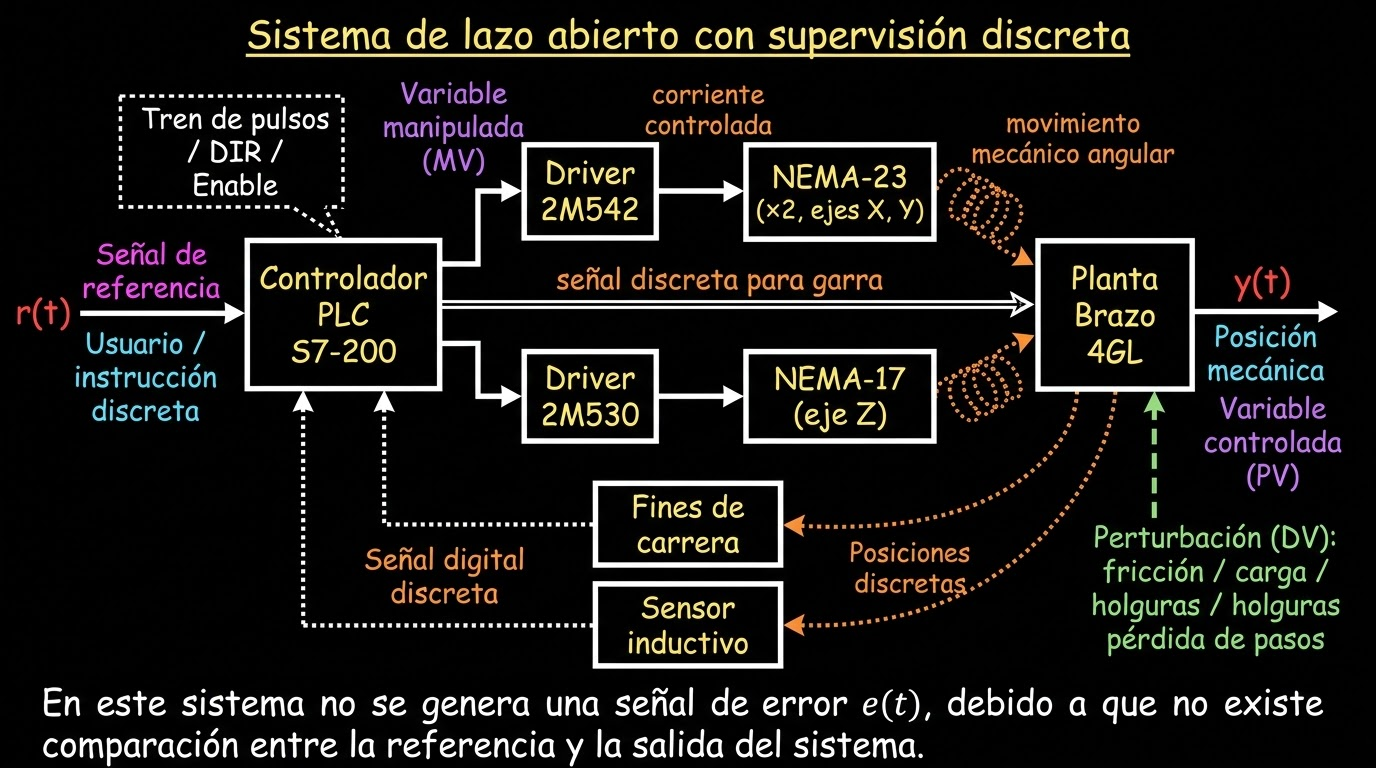
\includegraphics[width=0.85\linewidth]{diagrama_bloques_fenomenologico.png}
\caption{Diagrama de bloques fenomenológico del brazo (laboratorio 1).}
\end{figure}

\subsection{Arquitectura de datos de 3 capas}
\begin{figure}[H]
\centering
\begin{tikzpicture}[node distance=6mm and 22mm, every node/.style={font=\scriptsize}]
\node[cajab, text width=2.9cm] (c) {\textbf{Campo}\\PLC S7-200, sensores, drivers y motores};
\node[cajan, right=of c, text width=2.9cm] (m) {\textbf{Middleware}\\programa en la PC que lee los registros del PLC};
\node[cajab, right=of m, text width=2.9cm] (s) {\textbf{Servidor / cliente}\\base PostgreSQL, dashboard y HMI};
\draw[dflecha] (c) -- node[above]{PPI RS-485} node[below]{9600 bit/s} (m);
\draw[dflecha] (m) -- node[above]{SQL / HTTP} node[below]{JSON} (s);
\end{tikzpicture}
\caption{Recorrido de una variable: del sensor al registro binario del PLC, del middleware al motor relacional.}
\end{figure}
Con los requerimientos de persistencia acordados entre control y cómputo (PV, MV, alarmas y tiempos de operación) se dibujó el borrador del modelo entidad-relación que el laboratorio 3 formaliza.

\section{Laboratorio 2: planos normalizados v2.0 e interfaces}
\subsection{P\&ID versión 2.0 (ANSI/ISA-S5.1-2009)}
El P\&ID representa el brazo con los cuatro tipos de globo de la norma (campo, panel del operador, función compartida del PLC y pantalla compartida), señales de 0,25~mm y enlaces de proceso de 1,0~mm, y agrupa los instrumentos en cinco lazos:
\begin{center}\small
\begin{tabularx}{\linewidth}{c >{\raggedright}p{2.4cm} >{\ttfamily\raggedright\arraybackslash}X}
\toprule
\textbf{Lazo} & \textbf{Grado de libertad} & \textrm{\textbf{Tags ISA-5.1}}\\
\midrule
100 & general & HS-100, HS-100P, ZY-100, ZI-100\\
101 & base $\theta$ & ZS-101, HS-101A/B, ZIC-101, ZY-101\\
102 & carro X & ZSL/ZSH-102, HS-102A/B, ZIC-102, ZY-102\\
103 & carro Y & ZSL/ZSH-103, HS-103A/B, ZIC-103, ZY-103\\
104 & garra & HS-104, XC-104, XY-104, XV-104\\
\bottomrule
\end{tabularx}
\end{center}
\plano{brazo_pid_v2.pdf}{P\&ID versión 2.0 del brazo XK-JS1-1 (plano P\&ID-B4G-01).}

\subsection{Esquema eléctrico versión 2.0 (IEC 60617)}
Dos hojas, potencia y mando, con todos los bornes del PLC y de los drivers rotulados, números de cable, referencias cruzadas de los relés (convención hoja.columna) y 19 capas. La versión 2.0 corrige las discrepancias del laboratorio 1:
\begin{center}\small
\begin{tabularx}{\linewidth}{c >{\raggedright\arraybackslash}X}
\toprule
\textbf{Nº} & \textbf{Corrección verificada con el PLC en marcha}\\
\midrule
1 & Inductivo de la base en I0.0 y finales de carrera en I0.1--I0.4 (corrige la discrepancia 5).\\
2 & Tren de pulsos de X e Y desde una sola salida (Q0.1), repartido por K1 (Q0.5) y K2 (Q0.6).\\
3 & Salidas de dirección Q0.3 (X) y Q0.4 (Y) conectadas a DIR+ (discrepancias 3 y 4).\\
4 & Relé K3 redibujado: bobina por Q0.7 y contacto al solenoide (discrepancia 2).\\
5 & Pines de E/S completos en la tabla de E/S con tags ISA (discrepancia 1); Start en paralelo con S1 y Stop con S2.\\
6 & Drivers y motores identificados (2M542 / 2M530, NEMA 23 / NEMA 17) y nota de lazo abierto sin encoders (discrepancia 6).\\
\bottomrule
\end{tabularx}
\end{center}
Quedan marcados como SUPUESTO, para verificar con multímetro, el común de entradas 1M/2M, el nivel de PUL/DIR, la tabla DIP del 2M530 y la numeración del zócalo de los relés.

\subsection{Mockups, navegación y cuadro de campos}
El equipo de cómputo diseñó los dos entornos que pide la guía: la interfaz local de planta (aplicación en la PC, porque el brazo no tiene panel PanelView) y el dashboard del ERP web, con su organigrama de navegación (autenticación, interfaz local, dashboard). El cuadro de campos convierte diez elementos visuales en columnas de la base; por ejemplo, el selector de modo pasa a \codigo{estado\_io} de HS-100, el paro de emergencia a \codigo{orden} y \codigo{evento\_alarma}, y el tren de pulsos a \codigo{muestra} de SY-100.

\section{Laboratorio 3: control de versiones y modelo relacional}
\subsection{Repositorio y flujo de cambios}
Repositorio público: \url{https://github.com/GabAndGom/Brazo-de-4-grados-de-libertad}, con la jerarquía de la guía (\codigo{documentacion/planos\_isa/}, \codigo{documentacion/manuales\_inversa/}, \codigo{database/scripts/}) y una carpeta por laboratorio con su informe. El trabajo se organiza en ramas por componente (\codigo{feature/planos-v2-kaizen}, \codigo{feature/ladder-s7200-homing}, \codigo{feature/db-y-supervision}) que se integran en \codigo{main} mediante Pull Request revisado; el historial (\codigo{git log --oneline --graph}) se entrega en \codigo{git\_log.txt}.

\subsection{Modelo entidad-relación y lógico en 3FN}
El modelo guarda la telemetría histórica (PV y MV), los estados de las alarmas críticas y el registro de ingresos de los operadores, además del catálogo de la planta y las órdenes de control: 15 tablas en tercera forma normal.
\begin{figure}[H]
\centering
\includegraphics[page=7, width=\linewidth, trim=10mm 15mm 10mm 15mm, clip]{base_datos_brazo.pdf}
\caption{Modelo E-R conceptual: 15 entidades, relaciones 1:N y una M:N (orden--eje).}
\end{figure}
\begin{itemize}
\item \textbf{1FN}: cada variable es una fila de \codigo{variable} y cada medición una fila de \codigo{muestra}; los destinos de una orden van en \codigo{orden\_parametro}, uno por eje.
\item \textbf{2FN}: unidad y rango dependen solo de la variable; el modo, solo del ciclo de operación.
\item \textbf{3FN}: el rol depende del usuario, la severidad del tipo de alarma y la duración del ciclo se calcula en una vista.
\end{itemize}

\section{Trazabilidad entre control y cómputo}
El filtro de la fase 1 exige que el modelo de datos refleje la nomenclatura ISA de los lazos. El mismo tag identifica cada señal en todos los productos de la fase:
\begin{center}\small
\begin{tabular}{>{\ttfamily}l l l l}
\toprule
\textrm{\textbf{Tag}} & \textbf{P\&ID / eléctrico} & \textbf{PLC} & \textbf{Base de datos}\\
\midrule
ZS-101 & inductivo de la base & I0.0 & \codigo{punto\_io}\\
ZSL-102 / ZSH-102 & finales del carro X & I0.1 / I0.2 & \codigo{punto\_io}\\
ZY-100 & tren compartido X/Y & Q0.1 & \codigo{punto\_io}\\
ZY-102K / ZY-103K & relés K1 / K2 & Q0.5 / Q0.6 & \codigo{punto\_io}\\
XY-104 & relé de la garra K3 & Q0.7 & \codigo{punto\_io}\\
ZI-101 / ZI-102 / ZI-103 & posición de base, X, Y & cuenta de pulsos & \codigo{variable} (PV)\\
SY-100 / SY-101 & frecuencia de los trenes & PTO1 / PTO0 & \codigo{variable} (MV)\\
\bottomrule
\end{tabular}
\end{center}
Los 22 tags de señales y los 5 de variables continuas son únicos en la base (restricción UNIQUE) y cada uno conserva su lazo en \codigo{eje.lazo\_isa}.

\section{Hito y entregables de la fase 1}
\paragraph{Hito (fin de la semana 6): versión 2.0 corregida del P\&ID y del esquema eléctrico.} \textbf{Cumplido}: ambos planos están en DWG (AutoCAD 2018), DXF y PDF, con cajetín, tabla de revisión y las seis discrepancias corregidas.
\begin{center}\small
\begin{longtable}{>{\raggedright}p{6.6cm} >{\raggedright}p{1.8cm} >{\raggedright\arraybackslash}p{6.2cm}}
\toprule
\textbf{Entregable} & \textbf{Estado} & \textbf{Archivo (carpeta del laboratorio o de la guía 3)}\\
\midrule
\endhead
\multicolumn{3}{l}{\textbf{Laboratorio 1}}\\
Bitácora: ficha técnica, discrepancias, diagrama de bloques, arquitectura de 3 capas & \cumple & \codigo{informe\_lab01.pdf}\\
\multicolumn{3}{l}{\textbf{Laboratorio 2}}\\
P\&ID v2.0 (ISA-5.1) & \cumple & \codigo{brazo\_pid\_v2.dwg}\\
Esquema eléctrico v2.0 (IEC) & \cumple & \codigo{brazo\_electrico\_v2.dwg}\\
Mockups y organigrama & \cumple & \codigo{lab2\_mockups\_y\_organigrama.pdf}\\
Cuadro de campos & \cumple & \codigo{informe\_lab02.pdf}\\
\multicolumn{3}{l}{\textbf{Laboratorio 3}}\\
Enlace al repositorio & \cumple & repositorio en GitHub (portada)\\
Diagrama E-R y lógico en 3FN & \cumple & \codigo{base\_datos\_brazo.pdf}\\
Historial de cambios & \cumple & \codigo{git\_log.txt}\\
Informe de cierre de fase & \cumple & este documento\\
\bottomrule
\end{longtable}
\end{center}

\section{Conclusiones y continuidad}
\begin{enumerate}
\item La auditoría convirtió una documentación heredada incompleta en una base verificada: ficha técnica, seis discrepancias corregidas y planos v2.0 normados que se pueden regenerar y versionar.
\item La limitación principal de la planta quedó establecida desde la fase 1: sin sensor continuo de posición el brazo opera en lazo abierto con supervisión discreta. Las fases 2 y 3 parten de esta condición.
\item Control y cómputo comparten un solo lenguaje: los tags ISA del P\&ID son las claves de la base de datos, lo que permite que la telemetría de las fases siguientes sea trazable hasta el plano.
\item Para la fase 2 quedan por verificar en el tablero los puntos SUPUESTO del esquema eléctrico.
\end{enumerate}

\newpage
\section{Firmas del equipo e identificadores ORCID}
Los integrantes de la escuadra declaran que este informe recopila el trabajo de la fase 1 y lo firman con su identificador ORCID (\url{https://orcid.org}).
\begin{center}
\renewcommand{\arraystretch}{2.4}
\begin{tabular}{>{\raggedright}p{5.2cm} >{\raggedright}p{2.6cm} p{4cm} p{2.6cm}}
\toprule
\textbf{Integrante} & \textbf{Mención} & \textbf{ORCID} & \textbf{Firma}\\
\midrule
Gabriel Andres Gomez Calla & control & \hrulefill & \hrulefill\\
Jose Lenin Mamani Choque & control & \hrulefill & \hrulefill\\
Miguel Alejandro Lima Huarachi & control y cómputo & \hrulefill & \hrulefill\\
Román Abner Machicado Arequipa & control & \hrulefill & \hrulefill\\
Marco Eduardo Chura Rondo & cómputo & \hrulefill & \hrulefill\\
\bottomrule
\end{tabular}
\end{center}

\vspace{1.5cm}
\begin{center}
\begin{tabular}{c@{\hspace{2cm}}c}
\rule{6cm}{0.4pt} & \rule{6cm}{0.4pt}\\
Ing. Jorge Antonio Nava Amador & Auxiliar de docencia\\
Docente & \\
\end{tabular}
\end{center}

\end{document}
